\documentclass{article}


\usepackage{arxiv}
\usepackage{cite}
\usepackage[utf8]{inputenc} % allow utf-8 input
\usepackage[T1]{fontenc}    % use 8-bit T1 fonts
\usepackage{hyperref}       % hyperlinks
\usepackage{url}            % simple URL typesetting
\usepackage{booktabs}       % professional-quality tables
\usepackage{amsfonts}       % blackboard math symbols
\usepackage{nicefrac}       % compact symbols for 1/2, etc.
\usepackage{microtype}      % microtypography
\usepackage{lipsum}
\usepackage{graphicx}
%\includegraphics{image.png}
\usepackage{listings}
\usepackage{verbatim}

\graphicspath{ {./images/} }


\title{Essentials of Dart}


\author{
 Henry Nguyen \\
  Department of Computer Science\\
  University of Arizona\\
  Tucson, AZ 85721 \\
  \texttt{henryn098@email.arizona.edu} \\
  %% examples of more authors
   \And
 Adam Cunningham \\
  Department of Computer Science\\
  University of Arizona\\
  Tucson, AZ 85721 \\
  \texttt{laser@email.arizona.edu} \\
  \And

  %% \AND
  %% Coauthor \\
  %% Affiliation \\
  %% Address \\
  %% \texttt{email} \\
  %% \And
  %% Coauthor \\
  %% Affiliation \\
  %% Address \\
  %% \texttt{email} \\
  %% \And
  %% Coauthor \\
  %% Affiliation \\
  %% Address \\
  %% \texttt{email} \\
}

\begin{document}
\maketitle
\begin{abstract}

\end{abstract}


% keywords can be removed
%\keywords{First keyword \and Second keyword \and More}


\section{Introduction}

\section{History}
Dart first appeared in 2011 with Elixir and Kotlin. A year later, TypeScript was released by Microsoft. The language was essentially designed to solve the frustrations of JavaScript at the time. Created at Google by Lars Bak and Kasper Lund, Dart is an optionally typed object-oriented language.
Dart can act as a superset of JavaScript with the dart2js compiler which included optional static type analysis. Dart is known in the community as the JavaScript killer, partly due to the large increase in popularity of Flutter, Google’s UI framework for building native interfaces in iOS and Android.

\begin{figure}[h]
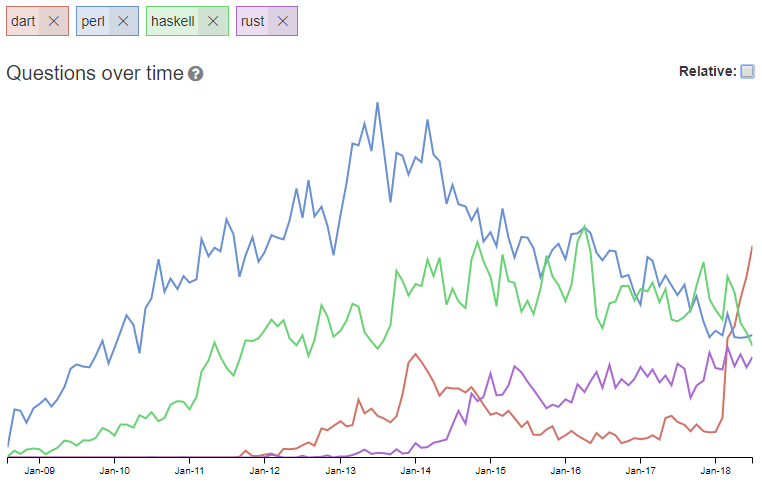
\includegraphics[scale=.45]{dart usage.png} \\
\textit {
The recent popularity of Dart, coupled with its ongoing support and use in upcoming Google projects makes Dart a compelling language
}
\end{figure}

Flutter is a major project that allows AOT (Ahead of time) and JIT (Just in Time) compilation. This leads to innovative development with hot-reload and a smoother UX. In addition, Flutter is able to render 120 fps on supported devices. Flutter is ran via the Dart platform, and Google is continuing to build and support Dart and Flutter. In 2016 Google began using dart to create a new operating system, Fuchsia, which is rumored to possibly replace the Android operating system.

\begin{comment}
\paragraph{Task modeling.}
We approach this task as a regression problem. For every item and shop pair, we need to predict its next month sales(a number).


\subsection{Headings: second level}
\lipsum[5]
\begin{equation}
\xi _{ij}(t)=P(x_{t}=i,x_{t+1}=j|y,v,w;\theta)= {\frac {\alpha _{i}(t)a^{w_t}_{ij}\beta _{j}(t+1)b^{v_{t+1}}_{j}(y_{t+1})}{\sum _{i=1}^{N} \sum _{j=1}^{N} \alpha _{i}(t)a^{w_t}_{ij}\beta _{j}(t+1)b^{v_{t+1}}_{j}(y_{t+1})}}
\end{equation}

\subsubsection{Headings: third level}
\lipsum[6]

\paragraph{Paragraph}
\lipsum[7]
\end{comment}

\section{Control Structures}
\label{sec:others}
\begin{comment}
\lipsum[8] \cite{kour2014real,kour2014fast} and see \cite{hadash2018estimate}.

The documentation for \verb+natbib+ may be found at
\begin{center}
  \url{http://mirrors.ctan.org/macros/latex/contrib/natbib/natnotes.pdf}
\end{center}
Of note is the command \verb+\citet+, which produces citations
appropriate for use in inline text.  For example,
\begin{verbatim}
   \citet{hasselmo} investigated\dots
\end{verbatim}
produces
\begin{quote}
  Hasselmo, et al.\ (1995) investigated\dots
\end{quote}

\begin{center}
  \url{https://www.ctan.org/pkg/booktabs}
\end{center}


\subsection{Figures}
\lipsum[10] 
See Figure \ref{fig:fig1}. Here is how you add footnotes. \footnote{Sample of the first footnote.}
\lipsum[11] 

\begin{figure}
  \centering
  \fbox{\rule[-.5cm]{4cm}{4cm} \rule[-.5cm]{4cm}{0cm}}
  \caption{Sample figure caption.}
  \label{fig:fig1}
\end{figure}

\begin{figure} % picture
    \centering
    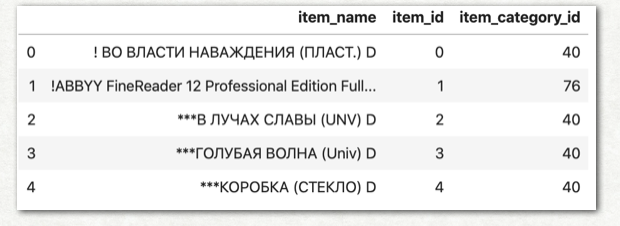
\includegraphics{test.png}
\end{figure}

\subsection{Tables}
\lipsum[12]
See awesome Table~\ref{tab:table}.

\begin{table}
 \caption{Sample table title}
  \centering
  \begin{tabular}{lll}
    \toprule
    \multicolumn{2}{c}{Part}                   \\
    \cmidrule(r){1-2}
    Name     & Description     & Size ($\mu$m) \\
    \midrule
    Dendrite & Input terminal  & $\sim$100     \\
    Axon     & Output terminal & $\sim$10      \\
    Soma     & Cell body       & up to $10^6$  \\
    \bottomrule
  \end{tabular}
  \label{tab:table}
\end{table}

\subsection{Lists}
\begin{itemize}
\item Lorem ipsum dolor sit amet
\item consectetur adipiscing elit. 
\item Aliquam dignissim blandit est, in dictum tortor gravida eget. In ac rutrum magna.
\end{itemize}
\end{comment}

\section{Data Types}
\label{sec:headings}
\begin{comment}
We are provided with five datasets from Kaggle: Sales train, Sale test, items, item categories and shops. In the Sales train dataset, it provides the information about the sales’ number of an item in a shop within a day. In the Sales test dataset, it provides the shop id and item id which are the items and shops we need to predict. In the other three datasets, we can get the information about item’s name and its category, and the shops’ name.
\paragraph{Task modeling.}
We approach this task as a regression problem. For every item and shop pair, we need to predict its next month sales(a number).
\paragraph{Construct train and test data.}
In the Sales train dataset, it only provides the sale within one day, but we need to predict the sale of next month. So we sum the day's sale into month's sale group by item, shop, date(within a month).
In the Sales train dataset, it only contains two columns(item id and shop id). Because we need to provide the sales of next month, we add a date column for it, which stand for the date information of next month.
\end{comment}

\section{Subprograms}
\begin{comment}
\label{sec:headings}
We are provided with five datasets from Kaggle: Sales train, Sale test, items, item categories and shops. In the Sales train dataset, it provides the information about the sales’ number of an item in a shop within a day. In the Sales test dataset, it provides the shop id and item id which are the items and shops we need to predict. In the other three datasets, we can get the information about item’s name and its category, and the shops’ name.
\paragraph{Task modeling.}
We approach this task as a regression problem. For every item and shop pair, we need to predict its next month sales(a number).
\paragraph{Construct train and test data.}
In the Sales train dataset, it only provides the sale within one day, but we need to predict the sale of next month. So we sum the day's sale into month's sale group by item, shop, date(within a month).
In the Sales train dataset, it only contains two columns(item id and shop id). Because we need to provide the sales of next month, we add a date column for it, which stand for the date information of next month.
\end{comment}

\section{Summary}
\label{sec:headings}
\begin{comment}
We are provided with five datasets from Kaggle: Sales train, Sale test, items, item categories and shops. In the Sales train dataset, it provides the information about the sales’ number of an item in a shop within a day. In the Sales test dataset, it provides the shop id and item id which are the items and shops we need to predict. In the other three datasets, we can get the information about item’s name and its category, and the shops’ name.
\paragraph{Task modeling.}
We approach this task as a regression problem. For every item and shop pair, we need to predict its next month sales(a number).
\paragraph{Construct train and test data.}
In the Sales train dataset, it only provides the sale within one day, but we need to predict the sale of next month. So we sum the day's sale into month's sale group by item, shop, date(within a month).
In the Sales train dataset, it only contains two columns(item id and shop id). Because we need to provide the sales of next month, we add a date column for it, which stand for the date information of next month.
\end{comment}
\bibliographystyle{plain}  
\bibliography{references}
\printbibliography
%%% Remove comment to use the external .bib file (using bibtex).
%%% and comment out the ``thebibliography'' section.


%%% Comment out this section when you \bibliography{references} is enabled.
%\begin{thebibliography}{1}

%\begin{comment}
%\newblock {\em arXiv fd arXiv:1804.09028}, 2018.
%\end{comment}
%\end{thebibliography}
\end{document}
